\setchapterpreamble[u]{\margintoc}
\chapter{Revolutionary for Whom?}
\labch{rev}

\textit{"The inhabitant of London could order by telephone, sipping his morning tea in bed, the various products of the whole earth -- he could at the same time and by the same means adventure his wealth in the natural resources and new enterprise of any quarter of the world -- he could secure forthwith, if he wished, cheap and comfortable means of transit to any country or climate without passport or other formality."} John Maynard Keynes, 1920 \cite{Keynes2012}

\section{Assistance from Assistants}

\textit{"Living off the wits of his subordinates - maybe that's leadership these days"}\cite{Lecarre}

You know, the whole concept of having an assistant has changed quite a bit over the years. In the old days, a well-to-do family might have employed a butler to help manage their estate, while nowadays, folks can simply use digital assistants like Siri or ChatGPT. But that's not all! There's also an interesting hybrid of sorts that has emerged in recent times – the Indian Virtual Assistant.

Now, if you think about it, traditional butlers were a sort of luxury. They cost a pretty penny and were thus reserved for the upper crust of society. On the other hand, these digital assistants – Siri, ChatGPT, and the like – well, they're pretty affordable, and just about anyone with a smartphone can access them. In a way, they've democratized assistance.

But there's another option that lies somewhere in between: the Indian Virtual Assistant. These human assistants, often based in India, provide remote support at a fraction of the cost of an in-person butler. They offer the human touch that digital assistants can't quite replicate, while still maintaining a certain level of affordability.

Now, don't get me wrong – I'm not saying digital assistants are bad. They're incredibly useful! But they've got some drawbacks, too. One concern is the potential for hacking and bugs. These AI-driven helpers are connected to the internet, and that means some folks with malicious intentions might try to break in and steal sensitive data. Plus, as impressive as machine learning can be, it's not perfect. Sometimes, these digital assistants might give you an answer that's a bit... off.

So, who might steer clear of AI assistants, despite their affordability and widespread availability? Well, for one, there are people who value their privacy and would rather not have a potential security risk handling their affairs. Then there are those who simply find comfort in human interaction, even if it means shelling out a little extra for a human assistant.

At the end of the day, the world of assistance has seen quite a revolution. As we navigate this new landscape, it's important to think about the trade-offs between cost, convenience, security, and the value of human expertise in the age of artificial intelligence.

\section{The Limitations of AI-generated Content}

\textit{"Another definition of modernity: conversations can be more and more completely reconstructed with clips from other conversations taking place at the same time on the planet.", "You are alive in inverse proportion to the density of cliches in your writing."}\sidecite{procrustes}

When it comes to AI-generated content, there's a certain fascination with the way machines can replicate human-like conversations. But are these AI-generated conversations truly akin to the ones between humans? Well, not exactly.

Let's take ChatGPT as an example. A recent article described it as a "Blurry JPEG of the Web" \sidecite{newyorkerChatGPTBlurry}, and that's quite an apt description. While AI models like ChatGPT are capable of generating coherent and contextually relevant responses, they often lack the depth and originality that genuine human conversations possess. In essence, AI-generated content can sometimes feel like a collage of borrowed ideas and phrases, strung together to mimic a conversation, but lacking the unique perspective and spontaneity that real human interaction entails.

Now, if we compare AI-generated content to traditional search engines, we can see some interesting differences. A search engine retrieves information from the vast expanse of the internet, presenting it to the user for their interpretation. An AI like ChatGPT, on the other hand, processes and generates content using a sophisticated regression model. But here's the catch: it might not always be right.

\textit{"(Traditional) search engines are databases, organized collections of data that can be stored, updated, and retrieved at will. (Traditional) search engines are indexes. a form of database, that connect things like keywords to URLs; they can be swiftly updated, incrementally, bit by bit (as when you update a phone number in the database that holds your contacts).}

\begin{marginfigure}[-5.5cm]
        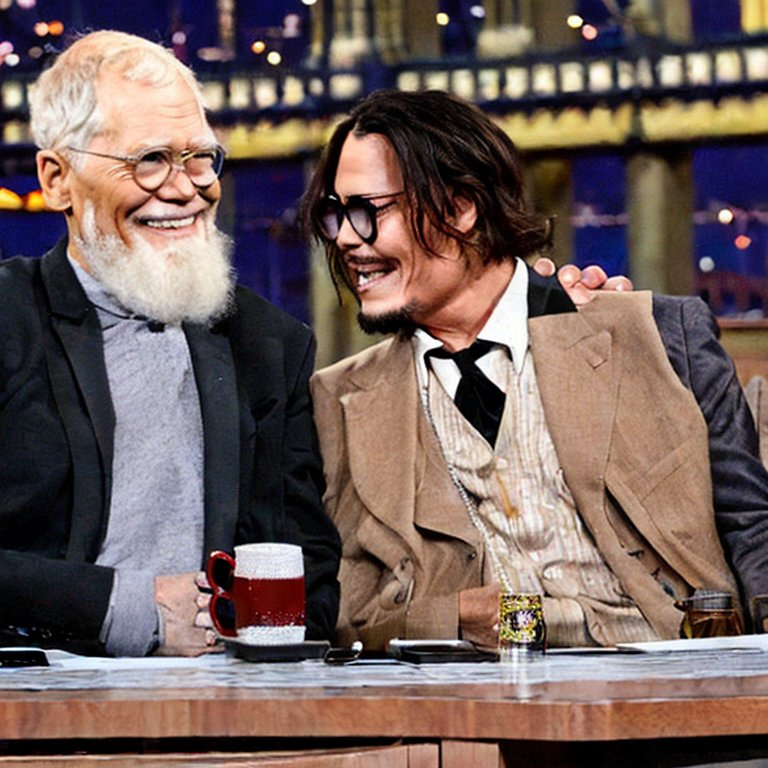
\includegraphics{depp}
        \caption{"david letterman laughing with johnny depp" made with Stable Diffusion 2.1}
        \labfig{depp}
\end{marginfigure}

\textit{Large language models do something very different: they are not databases; they are text predictors, turbocharged versions of autocomplete. Fundamentally, what they learn are relationships between bits of text, like words, phrases, even whole sentences. And they use those relationships to predict other bits of text. And then they do something almost magical: they paraphrase those bits of texts, almost like a thesaurus but much much better. But as they do so, as they glom stuff together, something often gets lost in translation: which bits of text do and do not truly belong together."} Gary Marcus, 2023 \sidecite{marcus2023}

In this sense, AI-generated content can be thought of as a creative interpretation of the information available to it. While it can provide valuable insights and answers, its limitations stem from its inability to truly comprehend the nuances of human conversation and thought. Consequently, the content produced may occasionally fall short in terms of accuracy, authenticity, or originality.

Therefore, as we continue to integrate AI-generated content into our lives, it's crucial to remember that these AI models, while impressive, are not perfect. They can offer valuable assistance, but they should not be treated as infallible sources of information or as substitutes for genuine human interaction.

\section{The AI Advantage in the Workplace}

There's a long-standing belief that human intelligence is unrivaled, and while it's true that humans possess unique capabilities, it's important to recognize the immense value AI can bring to the workplace.

Consider the humble calculator, for instance. Before its invention, humans would manually perform complex calculations, a process that was not only time-consuming but also prone to errors. The introduction of calculators transformed the way we approached mathematics, allowing us to quickly and accurately solve problems. Similarly, AI has the potential to revolutionize the way we work by handling tasks that would otherwise require significant time and effort from humans.

By embracing AI in daily tasks and careers, we can delegate responsibilities that computers excel at, such as processing large datasets, pattern recognition, and even language translation. This not only improves efficiency and accuracy but also frees up human workers to focus on tasks that require creativity, empathy, and critical thinking – areas where AI still falls short.

The key to reaping the benefits of AI in the workplace lies in finding the right balance between human expertise and AI capabilities. Rather than viewing AI as a threat to human intelligence, we should approach it as a powerful tool that complements and enhances our own skills. By working in tandem with AI, we can unlock new levels of productivity, innovation, and growth.

Ultimately, the integration of AI into the workplace offers countless opportunities for both individuals and organizations to thrive. By challenging the notion of superior human intelligence and acknowledging the strengths of AI, we can forge a harmonious partnership that drives success in the ever-evolving world of business.

\section{The "Organic Content" Market}

As AI becomes increasingly prevalent in content production, we may witness the emergence of a new market segment: handcrafted, 100\% organic content that is AI-free. This trend would be akin to the demand for organic, artisanal products in other industries, where consumers seek authenticity and the human touch.

The appeal of organic content lies in its perceived originality, creativity, and the assurance that it is the result of genuine human effort. This type of content may be highly sought after in industries such as journalism, literature, and the arts, where the value of human expression and unique perspectives is paramount.

However, the rise of this market also brings with it the potential for fraud. As AI-generated content becomes increasingly sophisticated and indistinguishable from human-generated content, distinguishing between the two may become a significant challenge. Unscrupulous individuals may attempt to pass off AI-generated content as organic, capitalizing on the demand for authentic human creations.

In order to combat fraud in the organic content market, it will be crucial to develop reliable methods for verifying the authenticity of content. This could include the use of digital signatures, blockchain technology, or other innovative solutions that provide a clear and tamper-proof record of a content's origin.

Moreover, fostering a culture of transparency and accountability within the content creation industry will be essential. By setting high ethical standards and encouraging open communication about the use of AI in content production, both creators and consumers can work together to ensure that the value of genuine human expression is preserved and celebrated.

\section{A Framework for Navigating AI's Impact on Careers}

In order to effectively navigate the impact of AI on careers, it is essential to develop a comprehensive framework that addresses the challenges and opportunities that arise from this technological revolution. The following framework can help navigate AI's impact on your business and career.

\subsection{Assess the Landscape}

\textbf{a. Identify AI-affected tasks:} Analyze your industry and job function to pinpoint tasks that are most likely to be influenced by AI. Consider which tasks are repetitive, data-intensive, or involve pattern recognition, as these are prime candidates for AI-driven automation.

\textbf{b. Evaluate AI maturity:} Assess the maturity of AI technologies relevant to your field, taking into account their current capabilities and potential future developments. This will help you gauge the timeline for AI adoption and its impact on job functions.

\subsection{Embrace AI as a Collaborator}

\textbf{a. Leverage AI for productivity:} Identify areas where AI can enhance your productivity by automating routine tasks, streamlining processes, or augmenting decision-making. Embrace AI as a tool that complements your skills and expertise, rather than a competitor.

\textbf{b. Cultivate human-centric skills:} Focus on developing skills that are uniquely human, such as creativity, empathy, critical thinking, and communication. These skills will remain valuable in the job market, even as AI becomes more pervasive.

\subsection{Adapt and Upskill}

\textbf{a. Pursue continuous learning:} Stay abreast of the latest AI advancements and their implications for your industry. Engage in lifelong learning through professional development courses, workshops, and industry events to maintain your competitiveness in the job market.

\textbf{b. Acquire AI-related skills:} Gain proficiency in AI-related skills, such as data analysis, machine learning, programming, or AI ethics. This will enable you to better understand and navigate the AI landscape, making you a more valuable asset to your organization.

\subsection{Shape the Future of Work}

\textbf{a. Advocate for responsible AI adoption:} Promote ethical AI implementation within your organization, addressing issues such as fairness, accountability, transparency, and privacy. Encourage the development of AI solutions that augment human capabilities, rather than replace them.

\textbf{b. Champion workforce transformation:} Support initiatives that facilitate workforce adaptation to AI, such as reskilling programs, mentorship opportunities, and the creation of new roles that leverage both human and AI strengths.

By following this framework, professionals can effectively navigate the impact of AI on their careers, seizing opportunities for growth and ensuring their continued success in the rapidly evolving world of work.

\section{Dead Inside}

\textit{"If you know, in the morning, what your day looks like with any precision you are a little bit dead - the more precision the more dead you are."}\sidecite{procrustes}

Conversational regression, or the tendency for AI-generated content to be a mere rehashing of existing ideas and phrases, can indeed result in rather monotonous and derivative interactions. In this sense, AI is, metaphorically speaking, "dead inside," lacking the spontaneity, creativity, and emotional depth that define human conversations.

While AI-powered tools like ChatGPT are impressive in their ability to generate coherent and contextually relevant responses, they cannot truly replicate the unique spark that arises from genuine human interaction. This is where we, as humans, can reclaim our strengths and embrace the richness of our own personalities and experiences.

Instead of attempting to imbue AI with the same emotional and intellectual depth as humans, we can leverage its strengths in areas such as data processing, pattern recognition, and automation, while focusing on cultivating our own unique skills and attributes. This approach allows us to maximize the potential of both AI and humans, enabling each to thrive in their respective domains.

So, let us embrace AI for what it is, a powerful tool that can enhance our lives and free us from mundane tasks. By doing so, we can devote more time and energy to the pursuits that make us truly human, be it creative endeavors, fostering deep connections with others, or simply exploring the world around us with curiosity and wonder.

In this way, we can create a harmonious balance between humans and AI, ensuring that we complement each other's strengths while preserving the very essence of what makes us alive.

\section{Go Forth and Procreate, Let The Calculators Multiply!}

To close I will address some concerns raised in an open letter signed by Elon Musk and Steve Wozniak in 2023 \sidecite{dumbestletter}. 

\subsection{Should we let machines flood our information channels with propaganda and untruth?}

The issue of propaganda and untruth in our information channels is not unique to AI-generated content. It is already a problem with state actors and other entities manipulating information. The solution lies in promoting media literacy and encouraging individuals to seek reputable news sources, such as the New York Times or the Wall Street Journal, rather than relying solely on social media for their information.

\subsection{Should we automate away all the jobs, including the fulfilling ones?}

Automation is a natural progression of technology, and it is impossible to regulate it away. If people find fulfillment in tasks that are automatable, they can still engage in these activities as hobbies or artisanal crafts. For example, they could open an Etsy shop and handcraft their products, or sharpen pencils by hand. Embracing AI and automation allows us to focus on more fulfilling, creative, and intellectually stimulating tasks that are uniquely human.

\subsection{Should we develop nonhuman minds that might eventually outnumber, outsmart, obsolete and replace us?}

The fear of AI outsmarting or replacing humans is based on the flawed assumption that being better at a single task implies complete superiority. AI systems may excel in specific domains, such as scoring high on standardized tests, but this does not mean they can replace humans altogether. The argument that AI will replace humans in the same way humans "replaced" our ape ancestors is misguided, as AI lacks the biological drive to procreate and compete. It is important to recognize that AI systems are tools designed to complement human abilities, not rivals seeking to supplant us.

\subsection{Should we risk loss of control of our civilization?}

\begin{marginfigure}[-5.5cm]
        
\includegraphics{jesus}
        \caption{"mdjrny-v4 a steampunk electronic Jesus saying "Go Forth and Multiply"" made with Mann-E}
        \labfig{jesus}
\end{marginfigure}

The notion of "losing control" of our civilization is a vague and misguided concern. Civilization is not a monolithic entity controlled by a single puppeteer but rather a complex, evolving system driven by the collective actions of individuals, communities, and institutions. Embracing AI does not mean relinquishing control over our society; instead, it provides us with powerful tools to shape our world and address the challenges we face. By integrating AI responsibly and ethically, we can harness its potential for the betterment of our civilization.

\section{Key Takeaways}

\begin{itemize}
\item \textbf{AI assistants aren't as good as butlers, but they are much cheaper} AI assistants, like ChatGPT and Siri, provide cost-effective and efficient alternatives to traditional butlers and virtual assistants, but users must consider potential drawbacks such as hackability and bugs.
\item \textbf{AI-generated content has limitations} While AI can produce content quickly and efficiently, it may lack the authenticity and depth of human-generated content, leading to a rise in the "organic content" market.
\item \textbf{Embrace AI in the workplace} AI tools can enhance productivity and allow humans to focus on more creative and intellectually stimulating tasks, similar to how calculators have transformed mathematical work.
\item \textbf{AI's "dead inside" nature} AI systems may be proficient at specific tasks, but they lack the human touch and personality, making it crucial for humans to focus on what we do best.
\item \textbf{Debunking AI misconceptions} AI is not a rival seeking to replace humans; instead, it is a powerful tool designed to complement human abilities and help shape our world.
\end{itemize}
